\documentclass[conference]{IEEEtran}

% Codificación y configuración general
\usepackage[utf8]{inputenc}
\usepackage[T1]{fontenc}
\usepackage[spanish,es-nodecimaldot]{babel}

% Paquetes habituales para artículos IEEE
\usepackage{cite}
\usepackage{amsmath,amssymb,amsfonts}
\usepackage{graphicx}
\usepackage{textcomp}
\usepackage{xcolor}
\usepackage{url}
\usepackage{booktabs}
\usepackage{listings}
\usepackage{algorithm}
\usepackage{algorithmic}

% TikZ para el diagrama a bloques
\usepackage{tikz}
\usetikzlibrary{shapes.geometric,positioning,arrows.meta}

\def\UrlBreaks{\do/\do-\do_}

\title{Experimentación Aprendizaje Supervisado: Autentificación de Billetes }

\author{
	\IEEEauthorblockN{Leonardo Daniel Aviña Neri}
	\IEEEauthorblockA{
		\texttt{ld.avinaneri@ugto.mx}
	}
	\and
	\IEEEauthorblockN{Diana Laura Garcia Zavala}
	\IEEEauthorblockA{
		\texttt{dl.garcia.zavala@ugto.mx}
	}
	\and
	\IEEEauthorblockN{Jonathan Omar Villafaña Razo}
	\IEEEauthorblockA{
		\texttt{jo.villafanarazo@ugto.mx}
	}
	\and
	\IEEEauthorblockN{Alejandro Reynoso Flores}
	\IEEEauthorblockA{
		\texttt{a.reynosoflores@ugto.mx}
	}
	\and
	\IEEEauthorblockN{Ademar Antonio De Leon Vazquez}
	\IEEEauthorblockA{
	\texttt{aa.deleonvazquez@ugto.mx
	}
	}
	\and
	\IEEEauthorblockN{Emmanuel Vargas Cisneros}
	\IEEEauthorblockA{
		\texttt{e.vargascisneros@ugto.mx}
	}
}

\begin{document}
	\maketitle
	
	\begin{abstract}
		En la autenticación de billetes los errores no cuestan lo mismo: aceptar una falsificación genera una pérdida económica, mientras que rechazar un billete genuino solo obliga a una revisión adicional. En este trabajo se comparan la regresión logística (modelo lineal usado como línea base) y el Random Forest (ensamble no lineal) con el conjunto \textit{Banknote Authentication}, de 1,372 billetes y cuatro características extraídas de imágenes. La pregunta es cuál identifica mejor los billetes falsos. La métrica principal, definida antes de comparar, es el recall de la clase falsa, acompañada de precisión, especificidad, $F_1$, exactitud y AUC. Se usó una partición 80/20 estratificada y los mismos cinco pliegues de validación cruzada para ambos modelos; el Random Forest se ajustó con validación anidada, se evitó la fuga de información y el conjunto de prueba se usó una sola vez. El recall por pliegue se comparó con una prueba $t$ pareada con la corrección de Nadeau y Bengio ($\alpha=0.05$). Ambos modelos obtuvieron un recall de 0.9959 en validación cruzada y de 1.0000 en prueba, y la prueba no rechazó $H_0$ ($p=1.0000$). Los falsos positivos difirieron (15 contra 10 en validación cruzada y 8 contra 1 en prueba), pero la desventaja de la regresión logística se concentra en billetes genuinos con un registro idéntico en el entrenamiento, por lo que no es concluyente. Con esta evidencia no se puede afirmar que un modelo sea mejor que el otro.
	\end{abstract}
	
	\begin{IEEEkeywords}
		autenticación de billetes, clasificación binaria, regresión logística, Random Forest, recall, validación cruzada anidada, corrección de Nadeau y Bengio
	\end{IEEEkeywords}
	
	\section{Introducción}
	% [TEXTO DE INTRODUCCIÓN OMITIDO]
	Hoy en día, el dinero representa uno de los activos o bienes aceptados de manera general como medio de pago para el intercambio de bienes o servicios, liquidar deudas personales o externas y medir el valor de los objetos. Esto no se limita al efectivo, ya que constituye un recurso disponible tanto en su forma física mediante billetes y monedas como digital, a través de los movimientos en la banca electrónica y el uso de criptomonedas como el Bitcoin. Su valor monetario se sustenta en una tasa regulada por cada país para su validación. 
	
	Sin embargo, desde la aparición del papel moneda, se han presentado situaciones donde diversas estrategias ilícitas para manipular o defraudar a las instituciones financieras permiten la circulación de piezas, lo que genera pérdidas reales de dinero para miles de usuarios y bancos. El empleo de tintas similares a las oficiales, la alteración de objetos para hacerlos pasar por piezas de alta denominación y la vulneración de códigos en cajas de seguridad figuran entre los problemas más comunes a los que se enfrenta el sector financiero global.
	En México se ha estimado que los billetes de 500 y 200 pesos son los más afectados por esta problemática. Esto evidencia cómo incluso las personas trabajadoras y honestas pueden convertirse en víctimas; la falta de conocimiento sobre el tema o el afán de obtener billetes de alta denominación facilitan las estafas a los comerciantes, quienes no solo pierden un ingreso, sino que suelen cargar con las consecuencias de estos delitos.
	\\\\
	Afortunadamente, el órgano institucional encargado de evaluar y ejecutar las políticas monetarias, el Banco de México proporciona información y guías de consulta para resolver tales incidentes. Entre las conclusiones destacan la necesidad de evaluar factores como la textura de la superficie del billete y la identificación de elementos visuales, símbolos y hologramas. Otras estrategias auxiliares incluyen el uso de bolígrafos con reactivos especiales que cambian de color al entrar en contacto con tintas no autorizadas y el empleo de dispositivos con luz negra para verificar la fluorescencia.
	
	El presente proyecto corresponde al análisis de una base de datos conformada por las propiedades matemáticas y estadísticas de billetes reales y falsos. Los registros, además de estar completos, corresponden a evaluaciones de billetes individuales.\\
	
	\begin{itemize}
		\item \textit{Pregunta de investigación}: \textbf{¿Cuál de los dos modelos de clasificación —la regresión logística como modelo lineal base y Random Forest como modelo no lineal— identifica mejor los billetes falsos, manteniendo un protocolo de evaluación estratificado, reproducible y libre de fuga de información?}\\
		\item \textit{Objetivo}: Determinar si dicha identificación automatizada es viable o si, por el contrario, se requiere un mayor volumen de información. El estudio busca dar respuesta a la interrogante y abrir la posibilidad de perfeccionar el modelo mediante la recopilación de datos y el análisis de más casos, con el fin de evaluar su vigencia a lo largo del tiempo y contribuir a la disminución de la tasa de fraudes en transacciones monetarias.\\
		\item\textit{ Alcance}: El estudio comprende el análisis exploratorio y computacional de los registros individuales contenidos en la base de datos disponible. Su propósito es evaluar la viabilidad matemática de la clasificación, sin llegar a implementar un sistema en tiempo real orientado a usuarios comerciales en esta fase inicial.
	\end{itemize}
	
	
	
	\section{Marco Teórico}
	% [SUBSECCIONES, IMÁGENES Y TEXTO DE METODOLOGÍA OMITIDOS]
	\subsection{Modelo 1: Regresión Logística}
	
	La regresión logística es un modelo discriminativo lineal basado en probabilidades, seleccionado como el primer clasificador para este espacio continuo de 4 dimensiones\cite{aws_logistic_regression}. Aunque comparte una estructura matemática similar a la regresión lineal, la regresión logística modela directamente la probabilidad posterior de la variable objetivo dado el vector de características predictoras $X$.
	
	Dada una observación $x = [x_1, x_2, x_3, x_4]^T$, correspondiente a las cuatro características extraídas, el modelo calcula un valor score $z$ definido como la combinación lineal de los datos y un vector de coeficientes $\beta$ (pesos y sesgo):
	
	\begin{equation}
		z = \beta_0 + \beta_1 x_1 + \beta_2 x_2 + \beta_3 x_3 + \beta_4 x_4
	\end{equation}
	
	Para mapear este valor arbitrario $z \in \mathbb{R}$ a un rango acotado de probabilidad $P(Y=1 | X) \in [0, 1]$, se aplica la función de activación sigmoide:
	
	\begin{equation}
		\sigma(z) = \frac{1}{1 + e^{-z}}
	\end{equation}
	
	Por ende, la probabilidad estimada $\hat{y}$ de que un billete sea clasificado como falso ($y=1$) toma la forma:
	
	\begin{equation}
		\hat{y} = P(y=1 | x) = \frac{1}{1 + e^{-(\beta_0 + \sum_{j=1}^{4} \beta_j x_j)}}
	\end{equation}
	
	Los parámetros del modelo $\beta$ se estiman minimizando la pérdida de Entropía Cruzada Binaria (\textit{Binary Cross-Entropy Loss}), equivalente a maximizar la función de log-verosimilitud del sistema sobre las observaciones de entrenamiento:
	
	\begin{equation}
		J(\beta) = -\frac{1}{m} \sum_{i=1}^{m} \left[ y^{(i)} \log(\hat{y}^{(i)}) + (1 - y^{(i)}) \log(1 - \hat{y}^{(i)}) \right]
	\end{equation}
	
	Donde $m$ representa el total de observaciones y $y^{(i)}$ es la etiqueta binaria real. Al no existir una solución analítica cerrada para minimizar esta función, se optimiza mediante métodos numéricos como L-BFGS\cite{aws_logistic_regression}.
	
	Para asignar una clase discreta, se evalúa la regla de decisión comparando la probabilidad estimada frente a un umbral $\tau$ (usualmente $0.5$):
	\begin{itemize}
		\item Si $\sigma(z) \ge \tau$, el billete se clasifica como falso.
		\item Si $\sigma(z) < \tau$, el billete se clasifica como genuino.
	\end{itemize}
	
	Este modelo lineal es idóneo para establecer una línea base y analizar el espacio de características de 4 dimensiones, permitiendo además evaluar el impacto de los errores asimétricos Falsos Positivos vs. Falsos Negativos a través de métricas como el \textbf{Recall}
	\\	\\	
	El Recall es la métrica con la que se comparan los dos modelos, y se selecciona porque la existencia del falso negativo es el error operacional más riesgoso, ya que se puede permitir que un billete falso pase como genuino produciendo que la tasa de error se dispare a medida que esos casos incrementan. Mientras que si el valor es más alto es porque detecta mejor las proporciones de las falsificaciones. 
	
	Lo cual hace que el resto de métricas pasen a segundo plano pues también deben colocar los casos posteriores como el conteo de genuinos así como los erróneamente asignados.
	
    \subsection{Modelo 2: Random Forest}
    \label{sec:rf}
    
    El segundo clasificador es un bosque aleatorio \cite{breiman2001random}. Para una observación $x\in\mathbb{R}^4$, el modelo construye $B$ árboles de decisión. Cada árbol $T_b$ se ajusta sobre una muestra bootstrap del entrenamiento: se extraen $n$ observaciones con reemplazo, de modo que una fracción aproximada de $e^{-1}\approx 0.368$ queda fuera de la muestra de ese árbol. En cada nodo no se evalúan las $p=4$ variables, sino un subconjunto aleatorio de tamaño $m$; con \texttt{max\_features='sqrt'} y $p=4$, se consideran $m=2$ predictores por corte. Esa doble aleatoriedad —bootstrap y selección de variables— reduce la correlación entre árboles y, con ella, la varianza del promedio \cite{hastie2009elements}. La implementación utilizada es la de scikit-learn \cite{pedregosa2011scikit}.
    
   Cada árbol produce una probabilidad $\hat{P}_b(y=1\mid x)$ para la clase falsa. El bosque promedia esas probabilidades y decide con umbral $0.5$:
    \begin{align}
    	\hat{P}_B(y=1\mid x) &= \frac{1}{B}\sum_{b=1}^{B}\hat{P}_b(y=1\mid x), \nonumber \\
    	\hat{y} &= \mathbb{1}\left\{\hat{P}_B(y=1\mid x)\ge 0.5\right\}.
    	\label{eq:rf-prob}
    \end{align}
    Aquí $y=1$ denota billete falso, igual que en el modelo lineal.
    
    Los cortes son de la forma $x_j\le t$ y se eligen maximizando la reducción de la impureza de Gini. Para un nodo $t$ con proporciones $p_{t0}$ y $p_{t1}$ de cada clase,
    \begin{equation}
    	G(t)=1-\sum_{k=0}^{1}p_{tk}^{2}.
    	\label{eq:gini}
    \end{equation}
    La reducción de impureza de un corte en la variable $j$ con umbral $t_0$ es
    \begin{equation}
    	\Delta G(t,j,t_0)=G(t)-\frac{n_L}{n_t}G(t_L)-\frac{n_R}{n_t}G(t_R),
    	\label{eq:delta-gini}
    \end{equation}
    donde $n_t$ es el número de observaciones del nodo y $n_L,n_R$ las de sus hijos. La contribución bruta de una variable al bosque suma, sobre todos los árboles, las reducciones $\Delta G$ de los nodos donde participa, ponderadas por el tamaño del nodo:
    \begin{equation}
    	\tilde{I}_j=\frac{1}{B}\sum_{b=1}^{B}\sum_{\substack{t\in T_b\\ v(t)=j}}
    	\frac{n_t}{n}\,\Delta G(t,j,t_0),
    	\label{eq:rf-importance-raw}
    \end{equation}
    donde $v(t)$ es la variable utilizada en el corte del nodo $t$.
    La importancia que reporta scikit-learn se obtiene normalizando la contribución de cada árbol y promediando entre árboles, lo que equivale en esencia a normalizar $\tilde{I}_j$ de modo que las $p$ variables reparten la unidad:
    \begin{equation}
    	I_j=\frac{\tilde{I}_j}{\sum_{k=1}^{p}\tilde{I}_k},
    	\qquad \sum_{j=1}^{p}I_j=1.
    	\label{eq:rf-importance}
    \end{equation}
    
    Esta medida describe qué variables usa el bosque, no una relación causal. Con predictores correlacionados, la importancia puede repartirse entre ellos; en este conjunto, \texttt{skewness} y \texttt{kurtosis} tienen una correlación aproximada de $-0.79$, por lo que sus valores deben leerse en conjunto.
    
    No se aplica \texttt{StandardScaler}. Los árboles no comparan distancias ni optimizan gradientes: solo ordenan los valores de cada variable para buscar umbrales. Una transformación monótona como $z=(x-\mu)/\sigma$ conserva el orden y, por tanto, los mismos cortes posibles. En un espacio de cuatro variables continuas, el bosque puede aproximar fronteras no lineales e interacciones sin imponer una forma funcional; el precio es que el modelo deja de ser una ecuación única y pasa a ser un conjunto de reglas.

    \subsection{Métricas de evaluación}
    \label{sec:metricas}
    
    Igual que en los modelos anteriores, la clase positiva es $y=1$ (billete falso) y la negativa es $y=0$ (genuino). Al comparar la clase real contra la predicha, cada billete cae en uno de cuatro casos, que se organizan en la matriz de confusión: verdaderos positivos ($TP$, falsificación detectada), verdaderos negativos ($TN$, genuino aceptado), falsos positivos ($FP$, genuino rechazado, que solo implica una revisión adicional) y falsos negativos ($FN$, falsificación aceptada como genuina, el error costoso). El enunciado de la práctica describe los errores en lenguaje de negocio (``aceptar una falsificación'', ``rechazar un genuino''); aquí se declara de forma explícita que la clase positiva es $y=1$ y que todas las métricas se calculan con esta convención. Las métricas usadas son:
    \begin{align}
    	\text{Recall} &= \frac{TP}{TP+FN}, \label{eq:recall}\\
    	\text{Especificidad} &= \frac{TN}{TN+FP}, \label{eq:espec}\\
    	\text{Precisión} &= \frac{TP}{TP+FP}, \label{eq:prec}\\
    	F_1 &= \frac{2\cdot\text{Precisión}\cdot\text{Recall}}{\text{Precisión}+\text{Recall}}, \label{eq:f1}\\
    	\text{Exactitud} &= \frac{TP+TN}{TP+TN+FP+FN}. \label{eq:acc}
    \end{align}
    
    El \textbf{recall} es la métrica principal. Es la proporción de falsificaciones que el modelo detecta, y su complemento, $FN/(TP+FN)$, es la tasa de falsificaciones aceptadas. La \textbf{especificidad} es el recall de la clase genuina y permite ver el costo operativo que el recall no muestra, pues cada genuino rechazado implica una revisión manual innecesaria. La \textbf{precisión} indica qué proporción de los billetes rechazados sí eran falsos, y el $F_1$ es la media armónica entre la precisión y el recall. La \textbf{exactitud} se reporta solo como referencia: aunque las clases están razonablemente balanceadas (55.5\,\% genuinos), un valor cercano a 99\,\% no indica cuántos errores hay ni de qué tipo, por lo que siempre se acompaña de los conteos $TN$, $FP$, $FN$ y $TP$.
    
    Todas estas métricas dependen del umbral $\tau$ que convierte la probabilidad estimada en una clase. Para evaluar qué tan bien ordena el modelo las probabilidades sin fijar $\tau$ se usa la curva ROC (\textit{Receiver Operating Characteristic}) \cite{fawcett2006roc}, que grafica para cada umbral la tasa de verdaderos positivos contra la de falsos positivos:
    \begin{equation}
    	\text{TPR}(\tau)=\frac{TP(\tau)}{TP(\tau)+FN(\tau)},\quad
    	\text{FPR}(\tau)=\frac{FP(\tau)}{FP(\tau)+TN(\tau)}.
    	\label{eq:roc}
    \end{equation}
    El área bajo la curva (AUC) resume la ROC en un solo número y se puede leer como una probabilidad: la de que un billete falso elegido al azar reciba una probabilidad mayor que un genuino elegido al azar \cite{hanley1982auc}. Un valor de 1 indica separación perfecta y 0.5 equivale al azar. Cada punto de la curva es un umbral distinto; en este estudio el punto de operación es $\tau=0.5$.
    
    \subsection{Validación cruzada estratificada}
    \label{sec:cv}
    
    En la validación cruzada de $k$ pliegues el conjunto de entrenamiento se divide en $k$ subconjuntos disjuntos. En cada iteración $i=1,\dots,k$ se ajusta el modelo con los otros $k-1$ pliegues y se mide una métrica $m_i$ en el pliegue $i$ \cite{kohavi1995study}. El resultado se resume con la media y la desviación estándar entre pliegues:
    \begin{equation}
    	\bar{m}=\frac{1}{k}\sum_{i=1}^{k}m_i,\qquad
    	s_m=\sqrt{\frac{1}{k-1}\sum_{i=1}^{k}(m_i-\bar{m})^2}.
    	\label{eq:cv-resumen}
    \end{equation}
    En la versión \textit{estratificada} cada pliegue mantiene la proporción de clases del conjunto completo, para que ninguna estimación dependa de que un pliegue tenga por casualidad muy pocos billetes falsos. Como cada observación se usa una sola vez como validación, también se obtiene una predicción fuera de muestra (\textit{out-of-fold}, OOF) para todos los billetes, y con ellas se calculan las métricas agrupadas, las matrices de confusión y las curvas ROC.
    
    Este esquema requiere dos precauciones. La primera es evitar la fuga de información: todo paso que aprenda de los datos, como el escalado o la búsqueda de hiperparámetros, se ajusta solo con el entrenamiento de cada pliegue (Secciones~\ref{sec:rf-metodologia} y~\ref{sec:exp}). La segunda es que los pliegues no son independientes, ya que los conjuntos de entrenamiento de dos pliegues cualesquiera comparten una fracción $(k-2)/(k-1)$ de los datos, es decir, 75\,\% con $k=5$. Por eso las $k$ estimaciones quedan correlacionadas y la varianza de su media se subestima, lo que hace que una prueba $t$ ordinaria sobre los pliegues sea optimista \cite{nadeau2003inference}. Esto motiva la corrección que se presenta en la Sección~\ref{sec:resultados}.
 
    \subsection{Trabajos relacionados}
    \label{sec:relacionados}
 
    Las características de este conjunto provienen de imágenes de especímenes genuinos y falsificados, digitalizadas con una cámara industrial de inspección de impresión, a las que se aplicó una transformada wavelet \cite{uci_banknote}. La extracción de rasgos de texturas de billetes con coeficientes wavelet fue descrita por un grupo del que forma parte V. Lohweg, donante del conjunto \cite{glock2009feature}.
 
    Otros trabajos han usado este conjunto para comparar clasificadores. Kumar et al. aplican seis algoritmos, entre ellos regresión logística y Random Forest, con tres proporciones de partición (80:20, 70:30 y 60:40), y reportan que algunos llegan a 100\,\% de exactitud según la proporción usada \cite{kumar2022fake}. 
    Easa et al. usan una máquina de vectores de soporte y reportan un desempeño muy alto \cite{easa2023fake}. Aboul-Yazeed y Hassanien evalúan cinco modelos (Random Forest, regresión logística, perceptrón multicapa, máquina de vectores de soporte y K-Star) después de aplicar selección de variables por correlación y por búsqueda \textit{best-first}, y reportan 99.7\,\% de exactitud para K-Star \cite{aboulyazeed2026enhanced}. Puri et al. entrenan un Random Forest con este conjunto, con una exactitud cercana a 99\,\%, y le extraen reglas si-entonces para explicar su comportamiento \cite{puri2017magix}.
 
    En los resúmenes que se consultaron, el desempeño se reporta sobre todo con la exactitud. Este trabajo cambia tres cosas: la métrica principal es el recall de la clase falsa, porque los errores no cuestan lo mismo, y las demás son complementarias; los dos modelos se comparan sobre los mismos pliegues, con validación anidada y sin fuga de información; y se hace un contraste estadístico explícito, con una corrección por el traslape de los conjuntos de entrenamiento \cite{nadeau2003inference}.

    
	\section{Metodología \& Preparación}
	El conjunto de datos utilizado en este estudio corresponde a \textit{Banknote Authentication}, una base de datos diseñada para la evaluación de modelos de clasificación en tareas de detección de fraude en papel moneda. Las observaciones provinieron originalmente de la digitalización de imágenes de billetes tanto genuinos como falsificados mediante cámaras fotográficas industriales de alta resolución. Con el propósito de reducir la dimensionalidad de las imágenes crudas y extraer descriptores cuantitativos significativos sobre la textura y los patrones del papel, se aplicaron transformaciones continuas de \textit{wavelets} (ondículas).
	
	El análisis exploratorio inicial permitió caracterizar la estructura del dataset, el cual está compuesto por un total de 1,372 observaciones y 5 variables, las cuales se detallan a continuación:
	
	\begin{itemize}
		\item \textbf{Variables predictoras (continuas):}
		\begin{itemize}
			\item \textbf{variance}: Varianza de la imagen transformada por \textbf{wavelet}, que mide la dispersión del contraste.
			\item \textbf{skewness}: Asimetría de la imagen transformada por \textbf{wavelet}, que cuantifica la falta de simetría en la distribución de tonos.
			\item \textbf{kurtosis}: Curtosis de la imagen transformada por \textbf{wavelet}, que evalúa la presencia de valores extremos en la textura.
			\item \textbf{entropy}: Entropía de la imagen original, la cual refleja el grado de aleatoriedad o información presente en el billete.
		\end{itemize}
		
	\end{itemize}
	
	
	Donde la variable objetivo es binaria por lo que solo posee 2 resultados posibles, representando los estados de que sea un billete genuino o si el billete es falso representado por el nombre de \texttt{is\_fake}.
	
	La auditoría de calidad de datos reveló los siguientes hallazgos estructurales clave:
	
	\begin{itemize}
		\item \textbf{Integridad:} No se detectaron valores nulos, faltantes, infinitos ni no numéricos en ninguna de las variables analizadas.
		\item \textbf{Duplicados:} Se identificaron 24 registros duplicados, los cuales se decidió conservar formalmente para preservar la distribución empírica original de los datos de entrenamiento.
		\item \textbf{Balance de clases:} La variable objetivo muestra una distribución equilibrada, compuesta por \textbf{762 billetes genuinos (55.54\%)} y \textbf{610 billetes falsos (44.46\%)}. Este equilibrio previene posibles sesgos en los clasificadores derivados de un desbalance severo de clases.
	\end{itemize}
	
	Para garantizar una evaluación rigurosa y prevenir la contaminación del conjunto de prueba durante el ciclo de modelado, el proceso de preparación de los datos se estructuró siguiendo criterios metodológicos estrictos orientados a la validez del experimento.
	
	En primer lugar, dada la naturaleza de las cuatro variables predictoras continuas extraídas por wavelets, se observó una heterogeneidad considerable en sus rangos y magnitudes. Puesto que algoritmos como la regresión logística dependen directamente de métodos de optimización basados en gradientes y en la magnitud del espacio vectorial, las diferencias de escala pueden provocar distorsiones en la convergencia del modelo o asignar un peso desproporcionado a variables con mayor varianza. Para corregir este comportamiento en la regresión logística, resulta indispensable aplicar un procedimiento de estandarización mediante \texttt{StandardScaler} sobre la totalidad de los descriptores numéricos \cite{datacamp_zscore}; el Random Forest, en cambio, no requiere escalado (Sección~\ref{sec:rf}). Esta transformación ajusta la escala de cada característica continua para centrar su media en cero y fijar su desviación estándar en la unidad:
	
	\begin{equation}
		z = \frac{x - \mu}{\sigma}
	\end{equation}
	
	En segundo lugar, con el fin de cumplir estrictamente la regla contra la fuga de datos, se garantizó la independencia absoluta entre los datos de ajuste y los de validación. Para lograrlo, el cálculo de la media ($\mu$) y de la desviación estándar ($\sigma$) mediante la función \texttt{scaler.fit()} se ejecutó de manera exclusiva sobre las observaciones del conjunto de entrenamiento correspondiente a cada pliegue de validación. Posteriormente, los parámetros obtenidos de dicho entrenamiento se aplicaron mediante la función \texttt{scaler.transform()} tanto al subconjunto de entrenamiento como al subconjunto de prueba externo. Bajo este esquema, el modelo nunca tiene acceso a estadísticas globales del conjunto de evaluación durante la fase de ajuste.
	
	Finalmente, para asegurar la total reproducibilidad del experimento en cualquier entorno computacional, se fijó de manera global la semilla aleatoria en 42 en cada una de las particiones de datos, pliegues de validación cruzada e inicialización de los clasificadores.
	% [SUBSECCIONES, IMÁGENES Y TEXTO DE RESULTADOS OMITIDOS]

    \subsection{Configuración experimental e hiperparámetros}
    \label{sec:rf-metodologia}
    
    Se parte del conjunto descrito en la sección anterior \cite{uci_banknote}. La configuración del Random Forest se mantuvo separada de la preparación de datos y no incluyó escalado. Para que la estimación sea reproducible y comparable con el resto del estudio, se fijó \texttt{random\_state=42}, una división 80/20 estratificada y un \texttt{StratifiedKFold} de 5 pliegues con \texttt{shuffle=True} sobre $X_{\text{train}}$. El conjunto $X_{\text{test}}$ no se usó en esta fase.
    
    Para cada pliegue externo, la selección de hiperparámetros se hizo con un bucle interno de 3 pliegues estratificados sobre el entrenamiento de ese pliegue. Se usó \texttt{GridSearchCV} con 48 combinaciones, producto de $2\times4\times3\times2$ valores (Tabla~\ref{tab:rf-grid}). La métrica de selección fue el recall medio de la clase falsa. Cuando varias combinaciones empataron en recall, se prefirió el mayor F1 de la clase falsa; si el empate persistió, se eligió la configuración más simple: menos árboles y menor profundidad. Este criterio se implementó en una función de refit que ordena las combinaciones con esos tres niveles.
    
    \begin{table}[t]
    	\centering
    	\caption{Rejilla de hiperparámetros del Random Forest.}
    	\label{tab:rf-grid}
    	\begin{tabular}{@{}p{0.32\linewidth}p{0.22\linewidth}p{0.40\linewidth}@{}}
    		\toprule
    		Hiperparámetro & Valores & Qué controla \\
    		\midrule
    		\texttt{n\_estimators} & 100, 300 & Número de árboles $B$; más árboles estabilizan el promedio. \\
    		\texttt{max\_depth} & 3, 5, 8, \texttt{None} & Profundidad máxima; limita la complejidad de cada árbol. \\
    		\texttt{min\_}\allowbreak\texttt{samples\_}\allowbreak\texttt{leaf} & 1, 3, 5 & Mínimo de observaciones por hoja; valores altos suavizan la frontera. \\
    		\texttt{max\_}\allowbreak\texttt{features} & \texttt{'sqrt'}, \texttt{None} & Variables evaluadas por corte; \texttt{'sqrt'} usa 2 de 4 y \texttt{None} usa las 4. \\
    		\bottomrule
    	\end{tabular}
    \end{table}
    
    La validación es anidada porque el bucle interno solo ve el entrenamiento del pliegue externo. El pliegue externo de validación no participa en la elección de hiperparámetros. Si la búsqueda se hiciera sobre los mismos datos que luego se reportan, la estimación quedaría sesgada por selección de modelo \cite{cawley2010overfitting,varma2006bias}. Al mantener separados ambos niveles, el desempeño externo estima cómo se comportaría el procedimiento completo —búsqueda incluida— ante datos no vistos. Después de recorrer los cinco pliegues, se repitió la búsqueda interna sobre todo $X_{\text{train}}$ y se ajustó el modelo final con los mejores hiperparámetros; ese modelo es el que se entrega para la evaluación externa, sin haber visto $X_{\text{test}}$.

    
	\section{Experimentación}
	\label{sec:exp}
	
	\subsection{Protocolo común a los dos modelos}
	
	Los dos clasificadores se evaluaron con exactamente el mismo protocolo, para poder comparar sus resultados pliegue contra pliegue. Con la semilla global \texttt{random\_state=42}, las 1,372 observaciones se dividieron de forma estratificada en 1,097 para entrenamiento y 275 para prueba (la proporción de billetes falsos es de 0.445 y 0.444, respectivamente). Sobre el entrenamiento se aplicó un \texttt{StratifiedKFold} de 5 pliegues con \texttt{shuffle=True}; cada pliegue de validación tiene 219 o 220 billetes, de los cuales aproximadamente 97 o 98 son falsos. Las posiciones de los pliegues se calcularon una sola vez y se reutilizaron para los dos modelos, así que cada par de resultados viene de los mismos billetes de validación.
	
	La regresión logística se ajustó con un \texttt{Pipeline} que tiene \texttt{StandardScaler} y \texttt{LogisticRegression} (\texttt{solver='lbfgs'}, \texttt{max\_iter=2000}), sin búsqueda de hiperparámetros. Como el escalador está dentro del \textit{pipeline}, se vuelve a ajustar en cada pliegue solo con su entrenamiento. El Random Forest siguió el esquema anidado de la Sección~\ref{sec:rf-metodologia}. En ambos casos la clase se asignó con el umbral $\tau=0.5$. En cada pliegue se calcularon exactitud, precisión, recall, especificidad, $F_1$ y AUC, junto con los conteos $TN$, $FP$, $FN$ y $TP$, y se resumieron con la media y la desviación estándar de los cinco pliegues. Las predicciones OOF de los cinco pliegues se agruparon para construir las matrices de confusión, las curvas ROC y el análisis de errores.
	
	\subsection{Verificación de las predicciones por pliegue}

La validación cruzada de la regresión logística solo devuelve las métricas de cada pliegue, así que se repitió el mismo procedimiento guardando las predicciones, y sus métricas y coeficientes finales coinciden con la tabla por pliegue de la regresión logística. En el Random Forest se verificó que sus pliegues contienen los mismos billetes de validación que los de la regresión logística, que sus etiquetas coinciden con el conjunto de datos y que el modelo final tiene los hiperparámetros reportados: \texttt{max\_depth=None}, \texttt{max\_features='sqrt'}, \texttt{min\_samples\_leaf=1} y \texttt{n\_estimators=300}. Con esto, las métricas recalculadas a partir de las predicciones de ambos modelos coinciden con sus tablas por pliegue.
	
	\subsection{Evaluación en el conjunto de prueba}
	
	Los dos modelos finales, ajustados con todo $X_{\text{train}}$, se evaluaron en $X_{\text{test}}$ una sola vez y con $\tau=0.5$. Ningún hiperparámetro, umbral ni criterio se eligió viendo estos resultados.
	
	\subsection{Procedimiento estadístico y de análisis de errores}
	
	La comparación estadística se hizo sobre el recall de la clase falsa por pliegue, usando la diferencia $d_i$ entre los dos modelos en cada uno de los cinco pliegues pareados. Se aplicó la prueba $t$ pareada con la corrección de Nadeau y Bengio como prueba principal y, solo como referencia, la $t$ pareada ordinaria, con $\alpha=0.05$ (los detalles están en la Sección~\ref{sec:resultados}). Para el análisis de errores se identificó cada billete mal clasificado, en validación cruzada y en prueba, con su tipo de error (FN o FP), su probabilidad estimada de ser falso y los valores de sus cuatro características, y además se contó cuántos billetes fallan en los dos modelos.
	
	Los 24 registros duplicados se conservaron y su efecto se midió aparte, como análisis de sensibilidad. El conjunto tiene 35 filas que pertenecen a 11 grupos de filas idénticas, todas de la clase genuina. Se contaron las filas de validación cuyo registro idéntico está en el entrenamiento de su mismo pliegue (23 de 1,097) y las filas de $X_{\text{test}}$ con un registro idéntico en $X_{\text{train}}$ (9 de 275), y se recalcularon las métricas sin ellas. Las tablas principales no se modifican.
	
	\subsection{Software y reproducibilidad}
	
	Los experimentos se ejecutaron con Python 3.13.14 y scikit-learn 1.9.1, junto con NumPy, pandas, SciPy y Matplotlib. Las mediciones por pliegue, las predicciones fuera de muestra, las predicciones de prueba, los billetes mal clasificados y el resultado de la prueba estadística se exportan en CSV y texto.

    
	\section{Resultados \& Análisis Estadístico}
	\label{sec:resultados}
	
	\subsection{Validación cruzada}
	
	La Tabla~\ref{tab:recall-folds} muestra el recall de cada modelo en los cinco pliegues pareados. Los dos promedian $0.9959\pm0.0056$: cada modelo acepta dos falsificaciones en total entre los 488 billetes falsos de entrenamiento (0.41\,\%), pero en pliegues distintos. En los demás indicadores, promediados por pliegue (media $\pm$ desviación estándar), el Random Forest obtiene valores algo mayores en precisión ($0.9801\pm0.0209$ frente a $0.9703\pm0.0153$), especificidad ($0.9835\pm0.0175$ frente a $0.9754\pm0.0130$) y $F_1$ ($0.9879\pm0.0131$ frente a $0.9829\pm0.0084$), pero las diferencias son menores que la desviación estándar entre pliegues de cada modelo.
	
	\begin{table}[t]
		\centering
		\caption{Recall de la clase falsa por pliegue y diferencia $d_i=R^{LR}_i-R^{RF}_i$ (mismos billetes de validación).}
		\label{tab:recall-folds}
		\footnotesize
		\begin{tabular}{@{}cccc@{}}
			\toprule
			Pliegue & Reg. logística & Random Forest & $d_i$ \\
			\midrule
			1 & 1.0000 & 1.0000 & $\phantom{-}0.0000$ \\
			2 & 0.9898 & 1.0000 & $-0.0102$ \\
			3 & 1.0000 & 0.9898 & $+0.0102$ \\
			4 & 0.9897 & 1.0000 & $-0.0103$ \\
			5 & 1.0000 & 0.9897 & $+0.0103$ \\
			\midrule
			Media & 0.9959 & 0.9959 & $\phantom{-}0.0000$ \\
			Desv. est. & 0.0056 & 0.0056 & $\phantom{-}0.0103$ \\
			\bottomrule
		\end{tabular}
	\end{table}
	
	La Tabla~\ref{tab:metricas} reúne las métricas calculadas con las 1,097 predicciones OOF agrupadas y con el conjunto de prueba. En validación cruzada la diferencia entre los modelos está en los falsos positivos: 15 genuinos rechazados con la regresión logística (2.46\,\% de los 609 genuinos) y 10 con el Random Forest (1.64\,\%). El AUC por pliegue es prácticamente igual en ambos modelos ($0.9997\pm0.0002$ y $0.9998\pm0.0002$) y muy cercano a 1, por lo que los dos ordenan casi perfectamente los billetes según su probabilidad de ser falsos.
	
	\begin{table}[t]
		\centering
		\caption{Métricas con $\tau=0.5$ en validación cruzada (OOF agrupado, 1,097 billetes) y en prueba (275 billetes). LR: regresión logística; RF: Random Forest.}
		\label{tab:metricas}
		\footnotesize
		\setlength{\tabcolsep}{3.5pt}
		\begin{tabular}{@{}lcccc@{}}
			\toprule
			& \multicolumn{2}{c}{Validación cruzada} & \multicolumn{2}{c}{Prueba} \\
			\cmidrule(lr){2-3}\cmidrule(lr){4-5}
			Métrica & LR & RF & LR & RF \\
			\midrule
			Recall (falsos) & 0.9959 & 0.9959 & 1.0000 & 1.0000 \\
			Precisión & 0.9701 & 0.9798 & 0.9385 & 0.9919 \\
			Especificidad & 0.9754 & 0.9836 & 0.9477 & 0.9935 \\
			$F_1$ & 0.9828 & 0.9878 & 0.9683 & 0.9959 \\
			Exactitud & 0.9845 & 0.9891 & 0.9709 & 0.9964 \\
			AUC & 0.99960 & 0.99979 & 0.99995 & 1.00000 \\
			\midrule
			$TN$ & 594 & 599 & 145 & 152 \\
			$FP$ & 15 & 10 & 8 & 1 \\
			$FN$ & 2 & 2 & 0 & 0 \\
			$TP$ & 486 & 486 & 122 & 122 \\
			\bottomrule
		\end{tabular}
	\end{table}
    
	\begin{figure}[t]
		\centering
		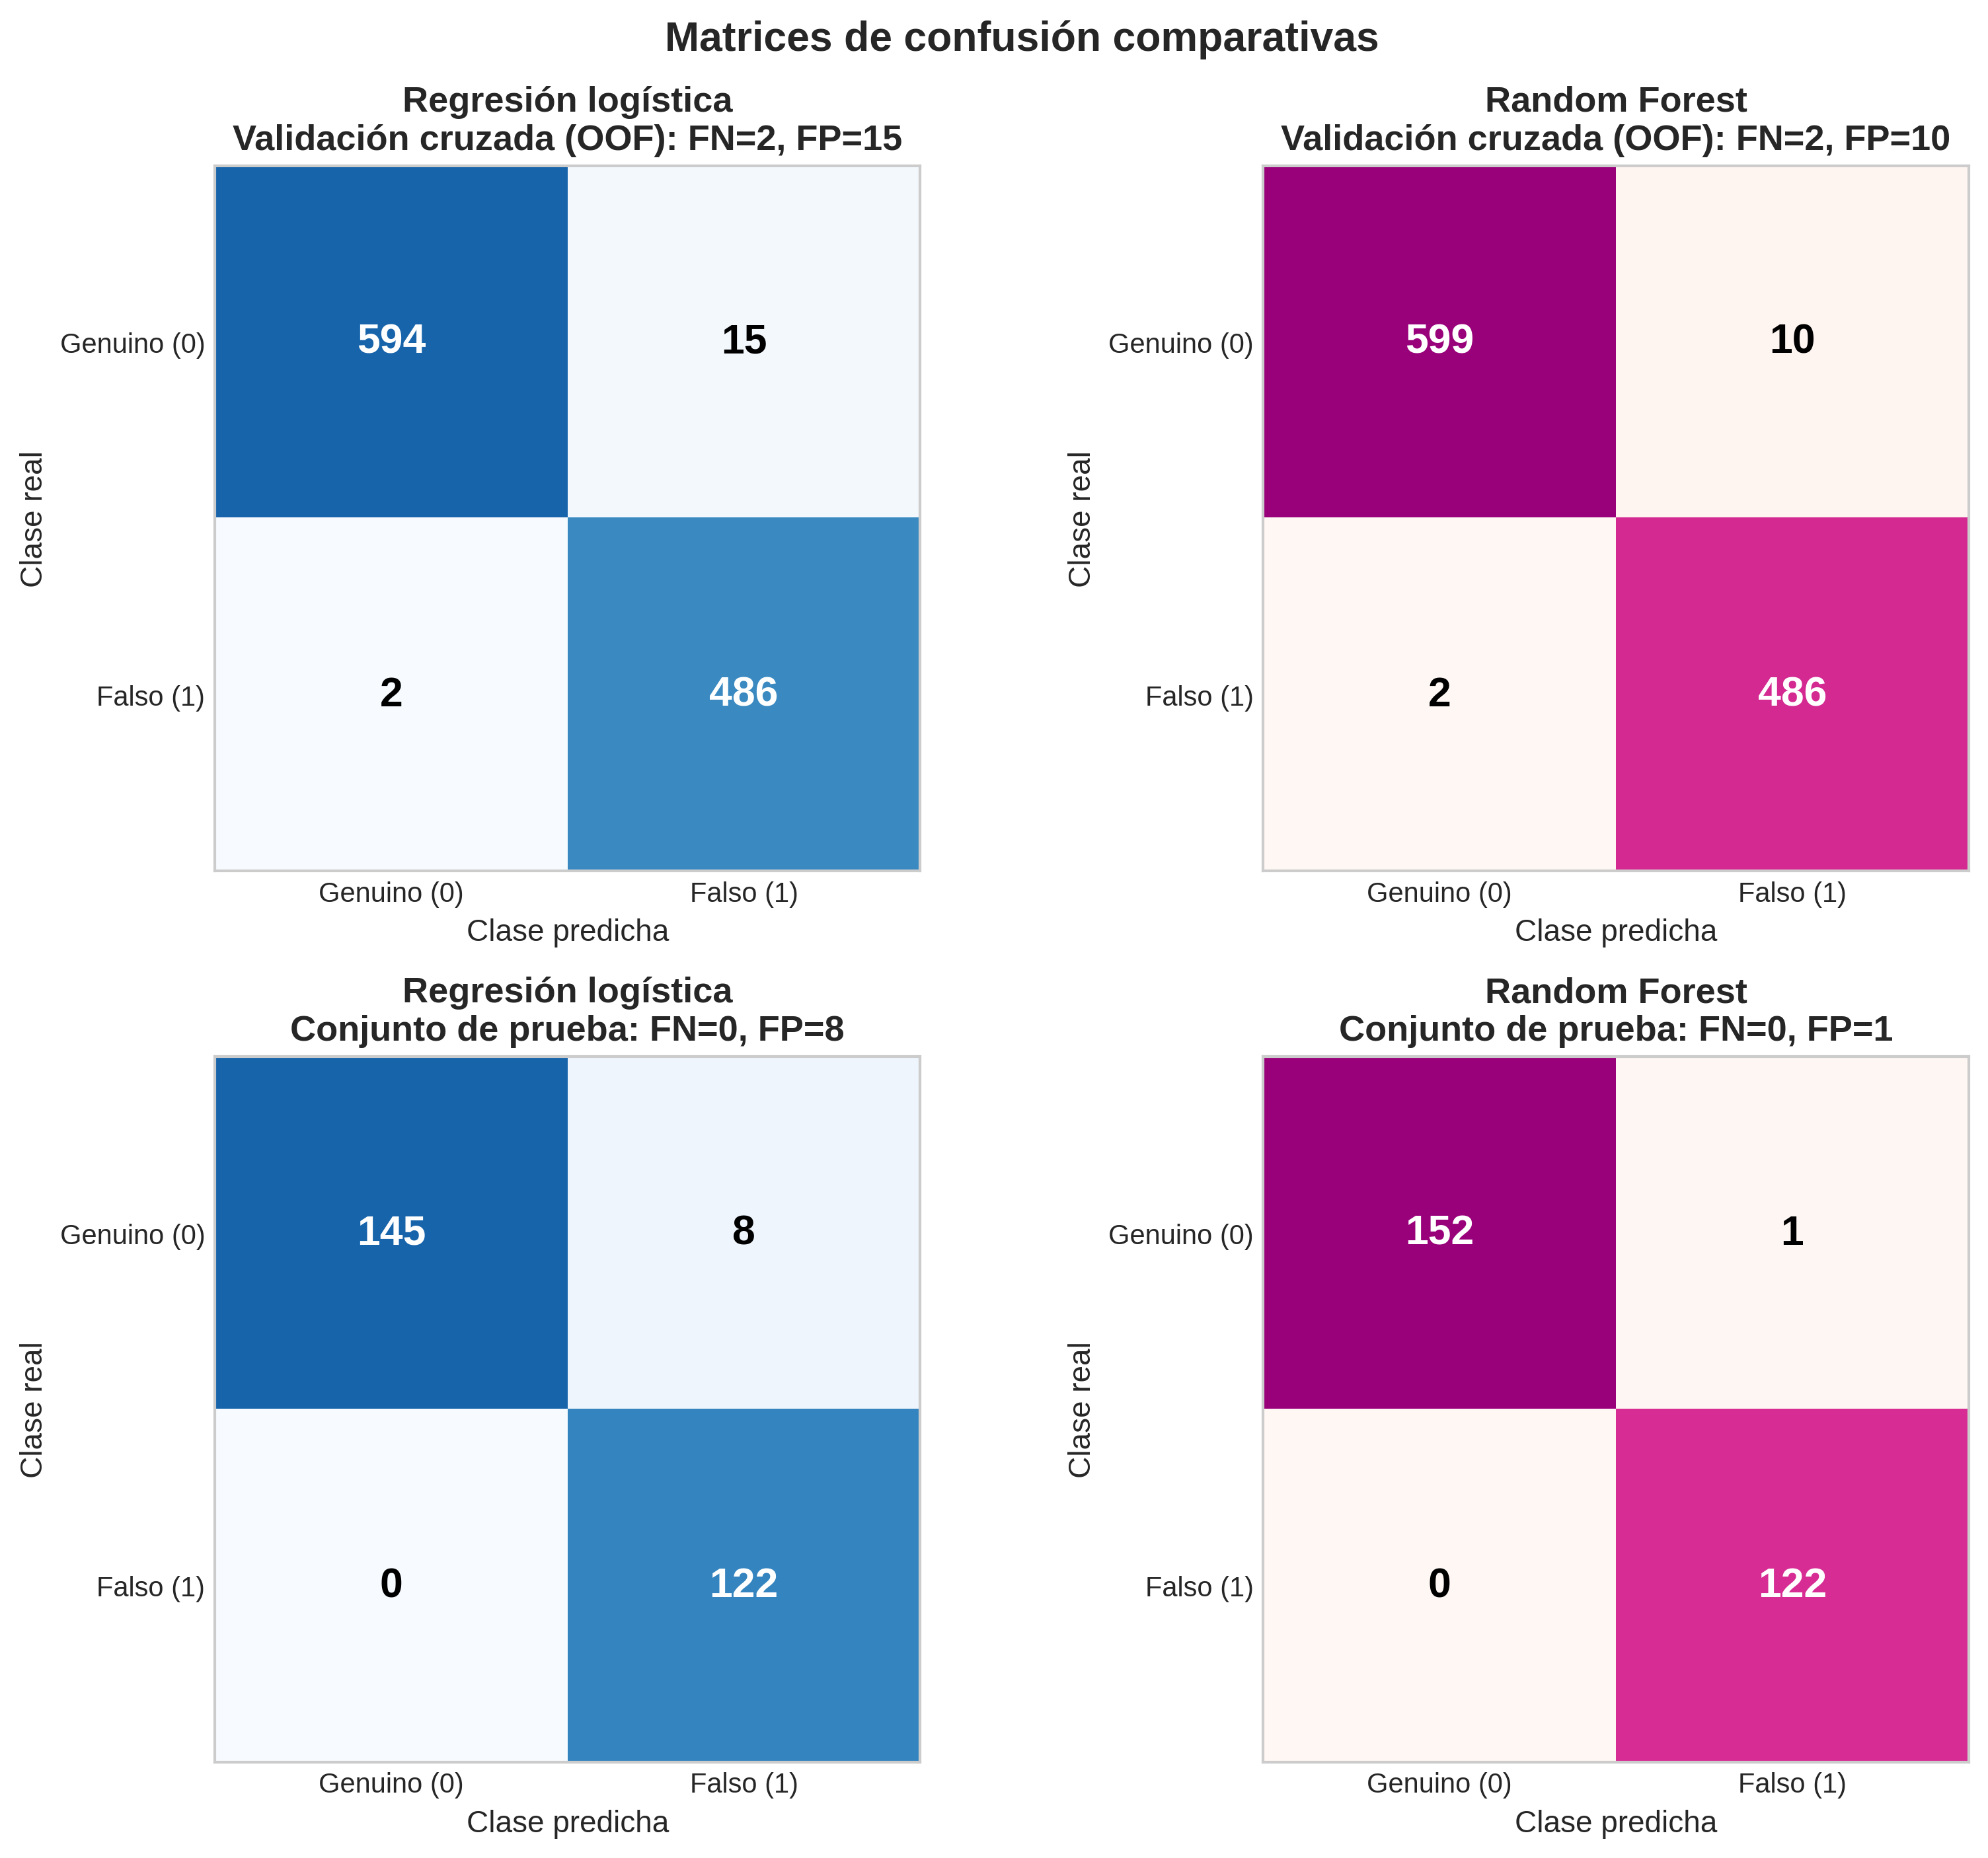
\includegraphics[width=\columnwidth]{plots/11_matrices_confusion_comparativas.png}
		\caption{Matrices de confusión de ambos modelos en validación cruzada (fila superior) y en el conjunto de prueba (fila inferior). La esquina inferior izquierda de cada matriz son los $FN$ (falsificaciones aceptadas) y la superior derecha los $FP$ (genuinos rechazados).}
		\label{fig:confusion}
	\end{figure}
	
	\begin{figure*}[t]
		\centering
		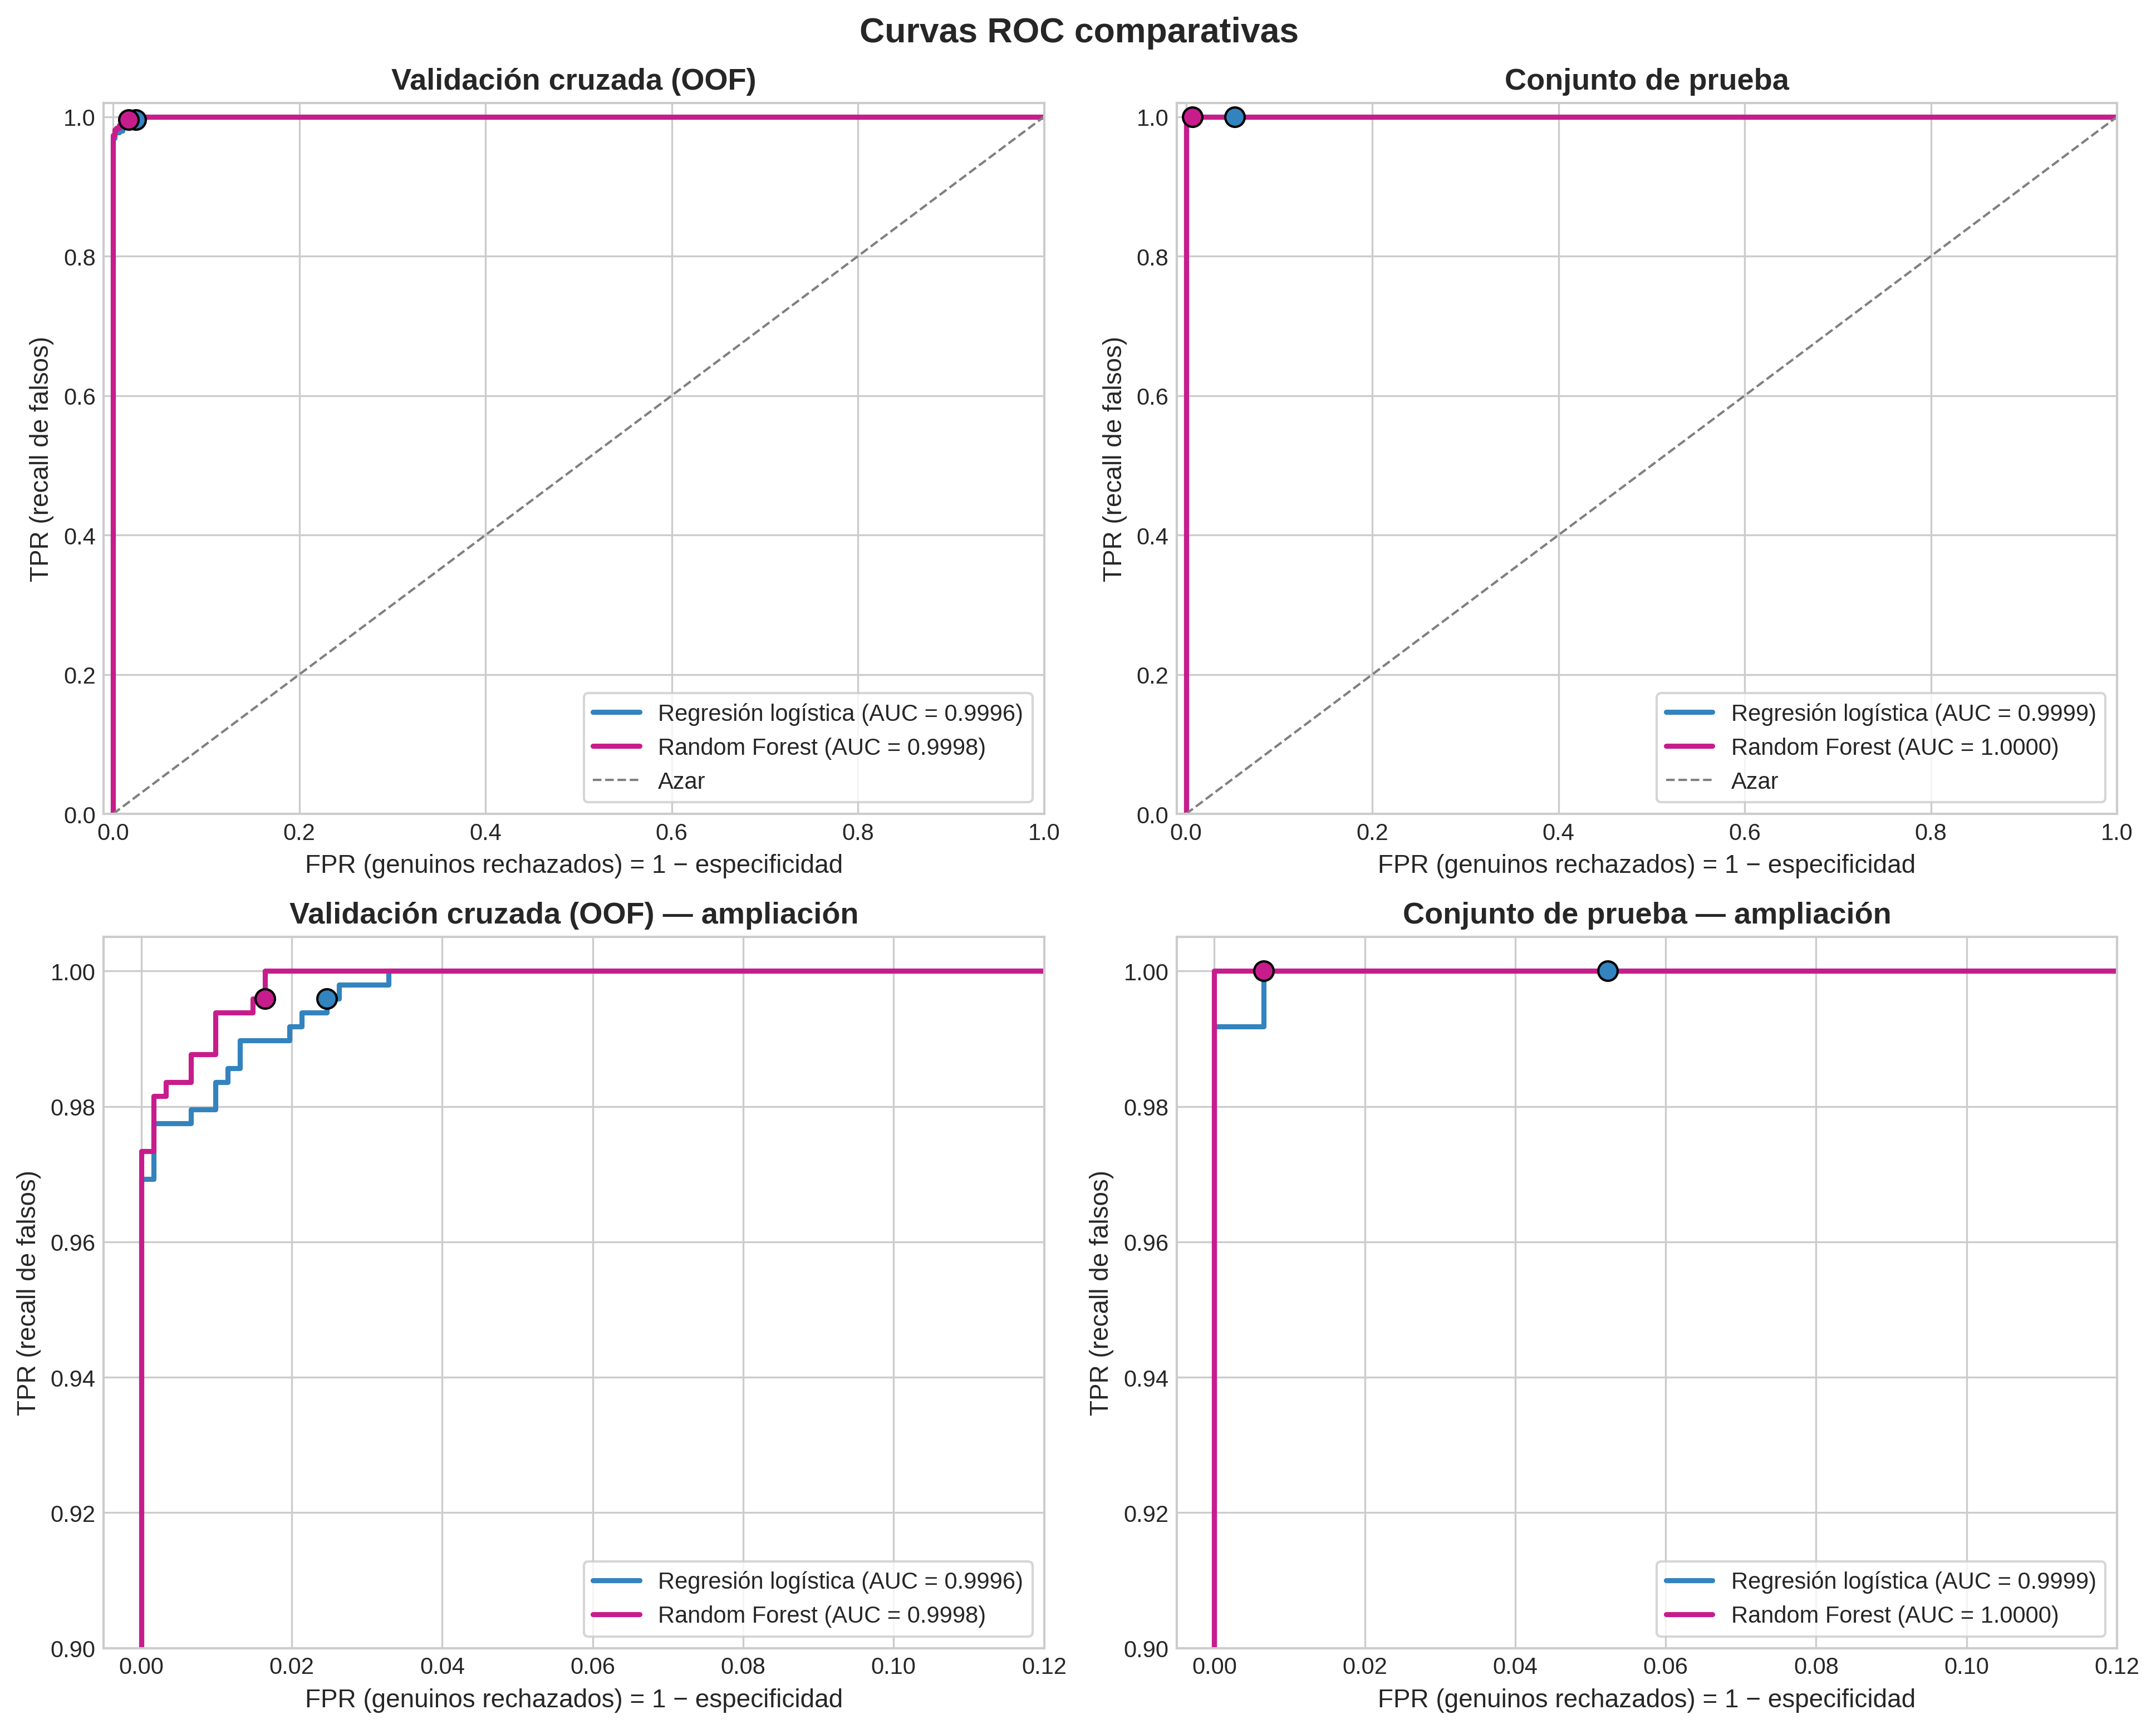
\includegraphics[width=0.78\textwidth]{plots/12_curvas_roc_comparativas.png}
		\caption{Curvas ROC y AUC de ambos modelos en validación cruzada (columna izquierda) y en prueba (columna derecha); la fila inferior amplía la esquina superior izquierda. El punto marcado es el umbral $\tau=0.5$. En validación cruzada la curva agrupa las probabilidades OOF de cinco modelos distintos, por lo que es una aproximación.}
		\label{fig:roc}
	\end{figure*}
	
	\subsection{Conjunto de prueba}
	
	En el conjunto de prueba (Tabla~\ref{tab:metricas} y Fig.~\ref{fig:confusion}) ninguno de los dos modelos acepta una falsificación: $FN=0$ de 122 billetes falsos. Las diferencias vuelven a aparecer en los falsos positivos, con 8 genuinos rechazados por la regresión logística contra 1 del Random Forest. Los AUC son $0.99995$ y $1.00000$ (Fig.~\ref{fig:roc}).
	
	\subsection{Prueba de hipótesis emparejada}
	
	La medida de rendimiento es el recall de la clase falsa en cada uno de los $k=5$ pliegues. Como los dos modelos se evaluaron en los mismos billetes, se trabaja con las diferencias pareadas $d_i=R_i^{LR}-R_i^{RF}$ de la Tabla~\ref{tab:recall-folds}.
	
	\textbf{Hipótesis y nivel de significancia.}
	\begin{equation}
		H_0:\ \mu_d=0 \qquad \text{frente a} \qquad H_1:\ \mu_d\neq 0,
	\end{equation}
	con $\alpha=0.05$. $H_0$ dice que el recall esperado de los dos modelos es el mismo. La prueba es bilateral, es decir, detecta diferencias en cualquier dirección.
	
	\textbf{Estadístico.} Con la media $\bar d=\frac{1}{k}\sum_i d_i$ y la desviación $s_d$ de las diferencias, la prueba principal es la $t$ pareada con la corrección de Nadeau y Bengio \cite{nadeau2003inference}, porque los entrenamientos de los pliegues se traslapan. La corrección cambia el factor $1/k$ por $1/k+n_{\text{prueba}}/n_{\text{entrenamiento}}$ en la varianza de $\bar d$:
	\begin{equation}
		t_c=\frac{\bar d}{\sqrt{\left(\frac{1}{k}+\frac{n_{\text{prueba}}}{n_{\text{entrenamiento}}}\right)s_d^{2}}},
		\label{eq:t-nb}
	\end{equation}
	con $k-1=4$ grados de libertad. Aquí $n_{\text{prueba}}/n_{\text{entrenamiento}}=0.250$, porque cada pliegue valida con una cuarta parte de los billetes que usa para entrenar. Como referencia se muestra la prueba $t$ pareada ordinaria, que no corrige esta dependencia:
	\begin{equation}
		t=\frac{\bar d}{s_d/\sqrt{k}}\ \sim\ t_{k-1}\quad\text{bajo }H_0.
		\label{eq:t-pareada}
	\end{equation}
	
	\textbf{Cálculo.} Con las diferencias de la Tabla~\ref{tab:recall-folds}, la media es $\bar d=0.0000$ y la desviación estándar es $s_d=0.01026$. La media no es un redondeo: los falsos negativos se cancelan exactamente, porque $d_2=-1/98$ y $d_3=+1/98$ (un $FN$ de la regresión logística en el pliegue 2 y uno del Random Forest en el 3), y $d_4=-1/97$ y $d_5=+1/97$ (un $FN$ de la regresión logística en el pliegue 4 y uno del Random Forest en el 5). Como el numerador es cero, $t=t_c=0$ sin importar el denominador. El error estándar ordinario es $s_d/\sqrt{5}=0.00459$ y el corregido es $\sqrt{1/5+0.25}\,s_d=0.00688$, es decir, 50\,\% mayor. Con el valor crítico $t_{0.975,\,4}=2.776$ se obtienen los intervalos de confianza de 95\,\% para $\mu_d$ de la Tabla~\ref{tab:prueba}.
	
	\begin{table}[t]
		\centering
		\caption{Resultado de la prueba sobre el recall ($\alpha=0.05$, 4 grados de libertad).}
		\label{tab:prueba}
		\footnotesize
		\begin{tabular}{@{}lccc@{}}
			\toprule
			Prueba & $t$ & $p$ & IC 95\,\% de $\mu_d$ \\
			\midrule
			$t$ con corrección N--B (principal) & $0.0000$ & $1.0000$ & $[-0.0191,\ +0.0191]$ \\
			$t$ pareada ordinaria (referencia) & $0.0000$ & $1.0000$ & $[-0.0127,\ +0.0127]$ \\
			\bottomrule
		\end{tabular}
	\end{table}
	
	\textbf{Supuestos.} (i) Pareo: se verificó que los billetes de validación de cada pliegue son los mismos para los dos modelos. (ii) Normalidad de las diferencias: con $k=5$ la prueba de Shapiro--Wilk ($W=0.8248$, $p=0.1270$) tiene muy poca potencia, por lo que solo se reporta como referencia. (iii) Independencia: no se cumple del todo por el traslape de 75\,\% entre entrenamientos, y por eso la prueba principal incluye la corrección. (iv) Resolución: con 97--98 falsificaciones por pliegue, un solo $FN$ mueve el recall aproximadamente $0.01$.
	
	\textbf{Decisión e interpretación.} Con $p=1.0000$ en las dos versiones no se rechaza $H_0$: estos datos no muestran diferencia en el recall de los modelos. Esto no demuestra que los modelos sean equivalentes. Los intervalos de confianza indican qué diferencias siguen siendo compatibles con los datos: hasta $\pm 0.019$ (con la corrección) en el recall medio, es decir, del orden de dos falsificaciones por pliegue.
	
	\textbf{Significancia práctica.} En billetes, y no en porcentajes, los dos modelos aceptan 2 falsificaciones de 488 (0.41\,\%) y difieren en 5 falsos positivos de 609 genuinos (15 frente a 10). La diferencia en falsos positivos es una métrica complementaria y no se contrastó con la prueba anterior, porque esa se definió solo para el recall.
	
	\subsection{Billetes mal clasificados}
	
	En validación cruzada los dos modelos cometen el mismo número de $FN$ (2 cada uno) y un número distinto de $FP$ (15 y 10), pero no fallan en los mismos billetes: ningún billete es mal clasificado por ambos modelos, ni como $FN$ ni como $FP$. Los 15 $FP$ de la regresión logística corresponden a 8 patrones de características distintos y los 10 del Random Forest a 10. La Tabla~\ref{tab:fn} lista los cuatro falsos negativos. Los de la regresión logística tienen características similares entre sí (\texttt{variance}\,$\approx 2.2$--$2.4$, \texttt{kurtosis}\,$\approx -5.0$), mientras que los del Random Forest son billetes distintos y de otra región del espacio de características. En los cuatro casos la probabilidad estimada de ser falso quedó entre $0.37$ y $0.50$, es decir, debajo del umbral pero sin ser claramente genuinos.
	
	\begin{table}[t]
		\centering
		\caption{Falsos negativos en validación cruzada (falsificaciones aceptadas). $\hat P$: probabilidad estimada de ser falso.}
		\label{tab:fn}
		\scriptsize
		\setlength{\tabcolsep}{2.5pt}
		\begin{tabular}{@{}lcccrrrr@{}}
			\toprule
			Modelo & Pl. & Índice & $\hat P$ & \texttt{var.} & \texttt{skew.} & \texttt{kurt.} & \texttt{entr.} \\
			\midrule
			LR & 2 & 1101 & 0.4359 & 2.1943 & 4.5503 & $-4.9760$ & $-2.7254$ \\
			LR & 4 & 918 & 0.3672 & 2.3917 & 4.5565 & $-4.9888$ & $-2.8987$ \\
			RF & 3 & 910 & 0.4389 & 0.5530 & $-3.4619$ & 1.7048 & 1.1008 \\
			RF & 5 & 1075 & 0.4950 & 0.3764 & $-0.8236$ & 0.7854 & 0.7452 \\
			\bottomrule
		\end{tabular}
	\end{table}
	
	En el conjunto de prueba no hay falsos negativos. Los 8 falsos positivos de la regresión logística corresponden a 6 patrones de características distintos: los índices 21 y 315 son idénticos, el 4 coincide con ellos salvo en la quinta cifra decimal de \texttt{variance} (0.32924 frente a 0.32920), los índices 170 y 498 son idénticos y los tres restantes son diferentes (345, 476 y 716). El único falso positivo del Random Forest (índice 95, $\hat P=0.7133$) no es un error de la regresión logística.
	
	\subsection{Efecto de los registros duplicados}
	
	De las 1,097 filas de validación, 23 (2.1\,\%) tienen un registro idéntico en el entrenamiento de su mismo pliegue, y 9 de las 275 filas de prueba tienen un registro idéntico en $X_{\text{train}}$; todas son de la clase genuina. Entre los errores, 10 de los 15 falsos positivos de la regresión logística en validación cruzada estaban en esa situación, y también 7 de los 8 de prueba. Ninguno de los 10 falsos positivos del Random Forest ni de los $FN$ de ningún modelo está en esa situación. La Tabla~\ref{tab:duplicados} compara las métricas con y sin esas filas.
	
	\begin{table}[t]
		\centering
		\caption{Análisis de sensibilidad: métricas con todas las filas y sin las filas que tienen un registro idéntico en el entrenamiento. El recall no cambia en ningún caso.}
		\label{tab:duplicados}
		\footnotesize
		\setlength{\tabcolsep}{3pt}
		\begin{tabular}{@{}llrcccc@{}}
			\toprule
			Conjunto & Modelo & $n$ & $FP$ & Precisión & Espec. & Exactitud \\
			\midrule
			\multicolumn{7}{@{}l}{\textit{Validación cruzada}} \\
			Todas & LR & 1097 & 15 & 0.9701 & 0.9754 & 0.9845 \\
			Todas & RF & 1097 & 10 & 0.9798 & 0.9836 & 0.9891 \\
			Sin copias & LR & 1074 & 5 & 0.9898 & 0.9915 & 0.9935 \\
			Sin copias & RF & 1074 & 10 & 0.9798 & 0.9829 & 0.9888 \\
			\midrule
			\multicolumn{7}{@{}l}{\textit{Prueba}} \\
			Todas & LR & 275 & 8 & 0.9385 & 0.9477 & 0.9709 \\
			Todas & RF & 275 & 1 & 0.9919 & 0.9935 & 0.9964 \\
			Sin copias & LR & 266 & 1 & 0.9919 & 0.9931 & 0.9962 \\
			Sin copias & RF & 266 & 1 & 0.9919 & 0.9931 & 0.9962 \\
			\bottomrule
		\end{tabular}
	\end{table}
	
	Los falsos positivos del Random Forest no dependen de estas filas: tiene 10 en validación cruzada y 1 en prueba con y sin ellas. Lo que cambia es la regresión logística. Al quitar las filas con registro idéntico, en el conjunto de prueba los dos modelos quedan con un solo $FP$ y métricas idénticas, y en validación cruzada la regresión logística pasa de 15 a 5 falsos positivos, por debajo de los 10 del Random Forest. Es decir, la desventaja aparente de la regresión logística en falsos positivos se concentra en filas con registro idéntico en el entrenamiento, y sin ellas la diferencia desaparece o se invierte. Esta comparación es descriptiva y no se contrastó estadísticamente. Dos filas con las mismas cuatro características y la misma clase son indistinguibles para el modelo, pero no se afirma que correspondan al mismo billete físico.

    
	\section{Discusión y Conclusiones}
	
	\subsection{Respuesta a la pregunta de investigación}
	
	La pregunta es cuál de los dos modelos identifica mejor los billetes falsos. Con la métrica principal, el recall de la clase falsa, no hay diferencia distinguible entre los modelos: los dos aceptan 2 falsificaciones de 488 en validación cruzada y ninguna de 122 en el conjunto de prueba, y la prueba de hipótesis no rechaza $H_0$ ($p=1.0000$, con o sin corrección). En la práctica, el modelo no lineal no aporta una mejora medible en la detección de falsificaciones respecto a la línea base lineal. Esto es coherente con que la regresión logística, de frontera lineal, ya ordena los billetes con un AUC de $0.9996$: el problema parece casi linealmente separable con estas cuatro características, por lo que la flexibilidad adicional del bosque tiene poco margen para aportar. En precisión y $F_1$ por pliegue el Random Forest obtiene valores algo mayores ($0.9801\pm0.0209$ frente a $0.9703\pm0.0153$ y $0.9879\pm0.0131$ frente a $0.9829\pm0.0084$), pero esas diferencias quedan dentro de la desviación estándar entre pliegues.
	
	\subsection{Tipos de error}
	
	Los dos tipos de error tienen consecuencias distintas. Los falsos negativos, que dejan pasar una falsificación, son los errores costosos, y son pocos y distintos en cada modelo: ningún billete falla en ambos. Las cuatro falsificaciones aceptadas tuvieron probabilidades entre 0.37 y 0.50, debajo del umbral de 0.5 pero cerca de él. Los falsos positivos, que solo generan revisiones manuales, sí distinguen a los modelos en números brutos (15 frente a 10 en validación cruzada y 8 frente a 1 en prueba). Sin embargo, la diferencia de la regresión logística se concentra en filas con registro idéntico en el entrenamiento (10 de sus 15 $FP$ en validación cruzada y 7 de sus 8 en prueba), mientras que los $FP$ del Random Forest son los mismos con y sin esas filas. Sin ellas la diferencia desaparece en prueba y se invierte en validación cruzada. Una hipótesis, que este trabajo no contrasta, es que el Random Forest, al no estar podado (\texttt{min\_samples\_leaf=1}), clasifica bien esos registros porque ya vio uno idéntico en el entrenamiento, mientras que la regresión logística, con su frontera lineal, no puede ajustarse a registros individuales. Por lo tanto, las diferencias en falsos positivos no son concluyentes y no deben presentarse como una ventaja del Random Forest.
	
	\subsection{Limitaciones}
	
	\begin{itemize}
		\item \textbf{Una sola semilla y una sola partición.} Se usó la semilla 42 y una partición 80/20; los resultados de prueba dependen de qué billetes quedaron en $X_{\text{test}}$ (275 billetes, 122 falsos).
		\item \textbf{Poca potencia estadística.} Con 5 pliegues y diferencias de uno o dos billetes por pliegue, la prueba solo detectaría diferencias grandes. El intervalo de 95\,\% de $\pm0.019$ para la diferencia en recall muestra que no se pueden descartar diferencias de hasta unas dos falsificaciones por pliegue. No rechazar $H_0$ no es lo mismo que probar equivalencia.
		\item \textbf{Prueba sobre una sola métrica.} Las diferencias que sí existen (falsos positivos) no se contrastaron, porque la métrica principal se fijó antes de ver los resultados y cambiarla después implicaría elegirla según el resultado.
		\item \textbf{Conjunto de prueba pequeño.} Con 0 falsos negativos en 122 falsificaciones, la regla de tres pone la tasa de falsas aceptaciones por debajo de aproximadamente $3/122\approx 0.025$ (2.5\,\%) con 95\,\% de confianza. No se puede afirmar que sea cero.
		\item \textbf{Duplicados.} Se conservaron, y 23 filas de validación tuvieron un registro idéntico en el entrenamiento de su pliegue. La detección usa igualdad exacta de los valores, así que los registros que difieren apenas en una cifra decimal no se detectan y el efecto podría estar subestimado. Una validación cruzada agrupada por registros idénticos evitaría el problema, pero cambiaría la partición común a los dos modelos.
		\item \textbf{Curva ROC agrupada.} En validación cruzada la curva junta las probabilidades de cinco modelos ajustados con datos distintos (y, en el bosque, con hiperparámetros que pueden ser distintos), por lo que es una aproximación.
		\item \textbf{Un solo conjunto de datos.} Los resultados no se pueden extrapolar a billetes de otras denominaciones, cámaras o épocas.
	\end{itemize}
	
	\subsection{Conclusiones}
	
	Los dos modelos detectan prácticamente todas las falsificaciones del conjunto: recall de $0.9959$ en validación cruzada y de $1.0000$ en prueba, sin diferencia estadísticamente detectable entre ellos. Las diferencias aparentes en falsos positivos se concentran en registros repetidos y desaparecen o se invierten al controlarlos, así que no son concluyentes. Como no hay diferencia distinguible en la métrica principal ni una ventaja sostenida en las demás, el modelo lineal, más simple e interpretable, es una opción razonable para este conjunto. Aun así, este experimento no permite declarar que un modelo sea mejor que el otro; la elección final depende de factores que aquí no se midieron, como el costo de las revisiones manuales y la necesidad de interpretar las decisiones. Como trabajo futuro se propone reducir los falsos negativos ajustando el umbral $\tau$ con un costo relativo explícito entre $FN$ y $FP$, seleccionado con datos de entrenamiento o validación y no con el conjunto de prueba; repetir la validación con particiones agrupadas por registros idénticos y con más semillas; y evaluar con más datos antes de cualquier uso operativo.
	
	\begin{thebibliography}{00}
    	\bibitem{aws_logistic_regression}
    	Amazon Web Services (AWS). 
    	\textit{¿Qué es la regresión logística?}. 
    	Disponible en: \url{https://aws.amazon.com/es/what-is/logistic-regression/} (Consultado en 2026).
    	
    	\bibitem{breiman2001random}
    	L. Breiman, ``Random forests,'' \textit{Machine Learning}, vol. 45, no. 1, pp. 5--32, 2001, doi: 10.1023/A:1010933404324.
    	
    	\bibitem{hastie2009elements}
    	T. Hastie, R. Tibshirani, and J. Friedman, \textit{The Elements of Statistical Learning: Data Mining, Inference, and Prediction}, 2nd ed. New York, NY, USA: Springer, 2009.
    	
    	\bibitem{pedregosa2011scikit}
    	F. Pedregosa \textit{et al.}, ``Scikit-learn: Machine learning in Python,'' \textit{J. Mach. Learn. Res.}, vol. 12, no. 85, pp. 2825--2830, 2011.
    	
    	\bibitem{datacamp_zscore}
    	DataCamp. 
    	\textit{¿Qué es la puntuación Z (Z-score) y cómo calcularla?}. 
    	Disponible en: \url{https://www.datacamp.com/es/tutorial/z-score} (Consultado en 2026).
    	
    	\bibitem{uci_banknote}
    	V. Lohweg, ``Banknote Authentication,'' UCI Machine Learning Repository, 2012, doi: 10.24432/C55P57. [Online]. Available: \url{https://archive.ics.uci.edu/dataset/267/banknote+authentication}
    	
    	\bibitem{cawley2010overfitting}
    	G. C. Cawley and N. L. C. Talbot, ``On over-fitting in model selection and subsequent selection bias in performance evaluation,'' \textit{J. Mach. Learn. Res.}, vol. 11, no. 70, pp. 2079--2107, 2010.
    	
    	\bibitem{varma2006bias}
    	S. Varma and R. Simon, ``Bias in error estimation when using cross-validation for model selection,'' \textit{BMC Bioinformatics}, vol. 7, art. 91, 2006, doi: 10.1186/1471-2105-7-91.
    	
    	\bibitem{fawcett2006roc}
    	T. Fawcett, ``An introduction to ROC analysis,'' \textit{Pattern Recognition Letters}, vol. 27, no. 8, pp. 861--874, 2006.
    	
    	\bibitem{hanley1982auc}
    	J. A. Hanley and B. J. McNeil, ``The meaning and use of the area under a receiver operating characteristic (ROC) curve,'' \textit{Radiology}, vol. 143, no. 1, pp. 29--36, 1982.
    	
    	\bibitem{kohavi1995study}
    	R. Kohavi, ``A study of cross-validation and bootstrap for accuracy estimation and model selection,'' in \textit{Proc. 14th Int. Joint Conf. Artificial Intelligence (IJCAI)}, 1995, pp. 1137--1143.
    	
    	\bibitem{nadeau2003inference}
    	C. Nadeau and Y. Bengio, ``Inference for the generalization error,'' \textit{Machine Learning}, vol. 52, no. 3, pp. 239--281, 2003.

        \bibitem{glock2009feature}
S. Glock, E. Gillich, J. Schaede, and V. Lohweg, ``Feature extraction algorithm for banknote textures based on incomplete shift invariant wavelet packet transform,'' in \textit{Pattern Recognition (DAGM 2009)}, J. Denzler, G. Notni, and H. S\"u{\ss}e, Eds., Lecture Notes in Computer Science, vol. 5748. Berlin, Germany: Springer, 2009, pp. 422--431, doi: 10.1007/978-3-642-03798-6\_43.

\bibitem{kumar2022fake}
P. V. Kumar, V. Akhila, B. Sushmitha, and K. Anusha, ``Detection of fake currency using KNN algorithm,'' \textit{Int. J. Res. Appl. Sci. Eng. Technol. (IJRASET)}, 2022, doi: 10.22214/IJRASET.2022.42829.

\bibitem{easa2023fake}
H. K. Easa, A. A. Saber, N. K. Hamid, and H. A. Saber, ``Machine learning based approach for detection of fake banknotes using support vector machine,'' \textit{Indones. J. Electr. Eng. Comput. Sci.}, vol. 31, no. 2, pp. 1016--1022, Aug. 2023, doi: 10.11591/ijeecs.v31.i2.pp1016-1022.

\bibitem{aboulyazeed2026enhanced}
R. S. Aboul-Yazeed and A. E. Hassanien, ``Enhanced banknote classification through machine learning and ensemble feature selection,'' in \textit{Proc. Int. Conf. Web 6.0 and Industry 6.0 (WIN 2025)}, S. Bhattacharyya \textit{et al.}, Eds., Lecture Notes in Networks and Systems, vol. 1508. Singapore: Springer, 2026, pp. 467--475, doi: 10.1007/978-981-96-8998-9\_37.

\bibitem{puri2017magix}
N. Puri, P. Gupta, P. Agarwal, S. Verma, and B. Krishnamurthy, ``MAGIX: Model agnostic globally interpretable explanations,'' arXiv:1706.07160, 2017.

    \end{thebibliography}
	
	\clearpage
	\onecolumn
	\appendices
	\section{Código Fuente}
	\label{app:codigo}
	
	El flujo reproducible se ejecuta con el archivo
	\texttt{code/main\_final.py}, que ejecuta en orden los notebooks
	\texttt{main.ipynb}, \texttt{main\_b.ipynb} y \texttt{main\_c.ipynb}.
	Los notebooks generan las figuras en \texttt{report/plots/} y los
	resultados experimentales en \texttt{results/pareja\_b/} y
	\texttt{results/pareja\_c/}. El archivo \texttt{repot.tex} es un borrador
	incompleto y no forma parte del documento final.
	
\end{document}